\documentclass{article}

% Margins.
\setlength{\oddsidemargin}{0in}
\setlength{\evensidemargin}{0in}
\setlength{\headheight}{12pt}
\setlength{\headsep}{42pt}
\setlength{\topmargin}{-54pt}
\setlength{\textwidth}{6.5in}
\setlength{\textheight}{9in}

\usepackage{float}
\usepackage{graphicx}

%opening
\title{Programming for Engineers I\\Lab 07\\For Loops}
\author{Hina Ashraf, Attique Dawood}

\begin{document}

\maketitle

\section{Loops (Repetition Statements)}
We have to calculate the sum of first 10 whole numbers i.e. add the numbers from 1 to 10. Following statement may be one way to do it.
\begin{verbatim}
    printf("Sum of first 10 numbers is = %d\n", 1+2+3+4+5+6+7+8+9+10);
\end{verbatim}
This method is perfectly fine as the syntax is right. The answer is also correct. This procedure can also be adopted while calculating the sum of numbers from 1 to 100. We can write the above statement adding all the digits from 1 to 100. But this method will not be suitable for computing the sum of numbers from 1 to 1000. The addition of a very big number of digits will result in a very ugly and boring statement. 


\section{For Loop}
The statements in the for loop repeat continuously for a specific number of times.  The while and do-while loops repeat until a certain condition is met.  The for loop repeats until a specific count is met.  Use a for loop when the number of repetition is known, or can be supplied by the user. 
The syntax of the for loop is as under:

\begin{verbatim}

for ( variable initialization; condition; variable update ) 
{
  Code to execute while the condition is true
}

\end{verbatim}

The Initialization is evaluated before the loop begins.  It is acceptable to declare and assign in the Initialization (such as int x = 1;).  This Initialization is evaluated only once at the beginning of the loop.
The testExpression will evaluate to TRUE (nonzero) or FALSE (zero).  While TRUE, the body of the loop repeats.  When the testExpression becomes FALSE, the looping stops and the program continues with the statement immediately following the for loop body in the program code.
The countExpression executes after each trip through the loop.  The count may increase/decrease by an increment of 1 or of some other value. 
Braces are not required if the body of the for loop consists of only ONE statement.  Please indent the body of the loop for readability.


% Flow Chart here
\begin{figure}[H]
\centering
\label{For-Loop-Flow-Diagram}
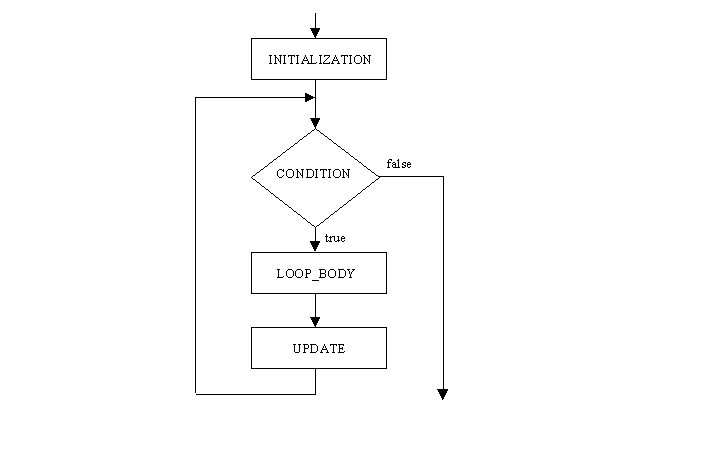
\includegraphics[width=1.0\textwidth]{For_Loop.PNG}
\caption{Flow diagram of for loop}
\end{figure}



\section{Exercise}
\textbf{Question No. 1:} Write a C++ code to print out all Armstrong numbers between 1 and 500. A number is called Armstrong number if sum of cubes of each digit of the number is equal to the number itself. For example $153=(1^3+5^3+3^3)$.\\
\textbf{Question No. 2:} Write a program to print the following shapes using for Loop (Take Height from the user). 

\begin{verbatim}
*           	*****               *       	 *****
**          	****               **       	  ****
***         	***               ***       	   ***
****        	**               ****       	    **
*****       	*               *****       	     *
\end{verbatim}
\end{document}
